\section{The effective potential of the superfluid and its minima}
\label{sec:potential}

\subsection{Definition}

The \emph{effective potential} $\Omega_{U2}(M_{U2},\Delta_{U2})$ is the expectation value of
$H^{\rm MF}_{U2}-\mu_{U2}N_{U2}$ per unit volume in the ground state of Eq.~\eqref{eq:HMF} at given
$M_{U2}$ and $\Delta_{U2}$, at zero temperature. That ground state fills, for every $\vec q$, the 16
negative eigenvalues of $\mathsf H_{U2}$, eight equal to $-E^+_{U2}$ and eight to $-E^-_{U2}$; with
no constant from the charge-symmetric order,
\begin{equation}
\Omega_{U2}=\frac{(M_{U2}-m_{U2})^2}{4G^S_{U2}}+\frac{|\Delta_{U2}|^2}{G^P_{U2}}
-8\int\frac{d^7q}{(2\pi)^7}\big(E^+_{U2}+E^-_{U2}\big).
\label{eq:Omega}
\end{equation}
The first two terms form the classical part $\Omega^{\rm cl}_{U2}$; the integral is the energy of
the filled states, measured from the chemical potential. Since
$\partial E^\pm_{U2}/\partial\Delta^*_{U2}=\Delta_{U2}/(2E^\pm_{U2})$ and
$\partial E^\pm_{U2}/\partial M_{U2}=(\varepsilon_{U2}\pm\mu_{U2})M_{U2}/(\varepsilon_{U2}E^\pm_{U2})$, the
conditions $\partial\Omega_{U2}/\partial\Delta^*_{U2}=0$ and $\partial\Omega_{U2}/\partial
M_{U2}=0$ are exactly the gap and the mass equations~\eqref{eq:gap}: \emph{the stationary points of
the effective potential are the self-consistent solutions of the self-interacting Dirac equation},
and the ground state is the global minimum. $\Omega_{U2}$ depends on $\Delta_{U2}$ only through
$|\Delta_{U2}|$ (R3-U1): a minimum at $\Delta_{U2}\neq0$ is a whole circle of minima in the complex
plane of $\Delta_{U2}$, the Mexican hat, and the choice of one point on it breaks $U(1)_{U2}$.

The integral diverges; the theory needs a cutoff $\Lambda_{U2}$ (Sec.~\ref{sec:status}), and all
numbers below are in units $\Lambda_{U2}=1$. We use two regularizations. \textbf{(R7)}: the length
$q$ of the seven-dimensional momentum is cut at $\Lambda_{U2}$; for an integrand that depends on $q$
only, $\int d^7q/(2\pi)^7(\dots)=a^{(7)}_{U2}\int_0^{\Lambda_{U2}}q^6(\dots)\,dq$ with
$a^{(7)}_{U2}=A_7/(2\pi)^7=1/(120\pi^4)$, where $A_7=16\pi^3/15$ is the area of the unit sphere in
seven dimensions. (R7) is used at every chemical potential. \textbf{(R8)}: in the vacuum the
fermion term is Lorentz invariant. The integral over the imaginary-time frequency
$\kappa^{(4)}_{U2}$ (the eighth component of the Euclidean momentum) of
$\ln[(\kappa^{(4)}_{U2})^2+(E^+_{U2})^2]/(2\pi)$ equals $E^+_{U2}$ up to a constant that does not
depend on $E^+_{U2}$; with it, $-16\int d^7q/(2\pi)^7(q^2+s_{U2})^{1/2}$ becomes
$-16\int d^8\kappa_{U2}/(2\pi)^8\ln(\kappa^2_{U2}+s_{U2})$, with $s_{U2}=M^2_{U2}+|\Delta_{U2}|^2$ and
$\kappa_{U2}$ the length of the Euclidean 8-momentum. Cutting $\kappa_{U2}$ at $\Lambda_{U2}$, and with
$a^{(8)}_{U2}=A_8/(2\pi)^8=1/(768\pi^4)$, $A_8=\pi^4/3$,
\begin{equation}
\begin{aligned}
\Omega_{U2}^{\rm (R8)}={}&\Omega^{\rm cl}_{U2}-8a^{(8)}_{U2}L_{U2}(s_{U2}),\\
L_{U2}(s_{U2})={}&2\int_0^1\kappa_{U2}^7\ln(\kappa_{U2}^2+s_{U2})\,d\kappa_{U2}\\
={}&\tfrac14(1-s_{U2}^4)\ln(1+s_{U2})+\tfrac14s_{U2}^4\ln s_{U2}\\
&-\tfrac1{16}+\tfrac1{12}s_{U2}-\tfrac18s_{U2}^2+\tfrac14s_{U2}^3,
\end{aligned}
\label{eq:OmegaR8}
\end{equation}
with the derivative $L'_{U2}(s_{U2})=\tfrac13-\tfrac12s_{U2}+s_{U2}^2-s_{U2}^3\ln[(1+s_{U2})/s_{U2}]$
(R3-P2; the closed form follows by one integration by parts). (R8) respects the Lorentz invariance
of the vacuum; (R7) does not, and the comparison of the two shows which results depend on the
regularization. In (R7) the vacuum integrals are elementary too: with
$\mathcal J^{(\iota)}_{U2}(s_{U2})=\int_0^1q^\iota(q^2+s_{U2})^{-1/2}dq$ for $\iota=0,2,\dots,8$,
$\mathcal J^{(0)}_{U2}=\ln[(1+(1+s_{U2})^{1/2})/s^{1/2}_{U2}]$,
$\iota\,\mathcal J^{(\iota)}_{U2}=(1+s_{U2})^{1/2}-(\iota-1)s_{U2}\mathcal J^{(\iota-2)}_{U2}$, and
$\int_0^1q^6(q^2+s_{U2})^{1/2}dq=\mathcal J^{(8)}_{U2}+s_{U2}\mathcal J^{(6)}_{U2}$ (R3-P1). In the
programs $\Omega_{U2}$ is computed relative to the normal state of mass $m_{U2}$ at the same
$\mu_{U2}$; this subtracts a constant and leaves the minima unchanged.

\subsection{The vacuum: the Mexican hat}

At $\mu_{U2}=0$, $E^+_{U2}=E^-_{U2}=(q^2+s_{U2})^{1/2}$, and the gap equation~\eqref{eq:gap}
reads $1/G^P_{U2}=8\int d^7q/(2\pi)^7(q^2+s_{U2})^{-1/2}$. Its right side decreases as $s_{U2}$
grows, so it has a root with $\Delta_{U2}\neq0$ only if $G^P_{U2}$ exceeds the value at
$s_{U2}\to0$, the \emph{critical coupling}
\begin{equation}
\begin{aligned}
G^{\rm crit}_{U2}&=\frac{3}{4a^{(7)}_{U2}}=90\pi^4\Lambda_{U2}^{-6}&&\text{(R7)},\\
G^{\rm crit}_{U2}&=\frac{3}{8a^{(8)}_{U2}}=288\pi^4\Lambda_{U2}^{-6}&&\text{(R8)},
\end{aligned}
\label{eq:Gcrit}
\end{equation}
(R3-P3: $8a^{(7)}_{U2}\int_0^1q^5dq=4a^{(7)}_{U2}/3$, and $8a^{(8)}_{U2}L'_{U2}(0)=8a^{(8)}_{U2}/3$). We
measure the couplings by $\lambda^P_{U2}=G^P_{U2}/G^{\rm crit}_{U2}$ and $\lambda^S_{U2}=4G^S_{U2}/
G^{\rm crit}_{U2}$; the factor 4 makes $\lambda^S_{U2}=1$ the critical value of the mass equation,
which at $m_{U2}=0$ reads $1/(4G^S_{U2})=8\int d^7q/(2\pi)^7(q^2+s_{U2})^{-1/2}$.

With $m_{U2}=0$ and without the scalar coupling ($M_{U2}=0$): for $\lambda^P_{U2}<1$ the minimum is
$\Delta_{U2}=0$ in both regularizations (R3-P5); for $\lambda^P_{U2}>1$ the minimum is at
$\Delta_{U2}\neq0$ and $\Delta_{U2}=0$ is a local maximum (R3-P4, 102 values of $\lambda^P_{U2}$ up to
3). Near the critical coupling the expansion of Eq.~\eqref{eq:Omega} in $\Delta_{U2}$ gives the Landau
form of the Mexican hat,
\begin{equation}
\begin{aligned}
\Omega_{U2}(\Delta_{U2})-\Omega_{U2}(0)={}&\tfrac43a^{(7)}_{U2}\Big(\frac1{\lambda^P_{U2}}-1\Big)|\Delta_{U2}|^2\\
&+\tfrac12a^{(7)}_{U2}|\Delta_{U2}|^4+\dots\quad\text{(R7)},
\end{aligned}
\label{eq:landau}
\end{equation}
from $(q^2+|\Delta_{U2}|^2)^{1/2}=q+|\Delta_{U2}|^2/(2q)-|\Delta_{U2}|^4/(8q^3)+\dots$ under
$\int_0^1q^6dq$ (the expansion fails only at $q\lesssim|\Delta_{U2}|$, which changes the next order,
$|\Delta_{U2}|^6\ln|\Delta_{U2}|$). The minimum is at
\begin{equation}
\begin{aligned}
|\Delta_{U2}|^2&=\tfrac43\big(1-1/\lambda^P_{U2}\big)&&\text{(R7)},\\
|\Delta_{U2}|^2&=\tfrac23\big(1-1/\lambda^P_{U2}\big)&&\text{(R8)},
\end{aligned}
\label{eq:landaugap}
\end{equation}
the second from $L_{U2}(s_{U2})=L_{U2}(0)+s_{U2}/3-s_{U2}^2/4+\dots$ (R3-P6: ratio of the computed
gap to these forms at $\lambda^P_{U2}=1.0005$ within 1 per cent). Figure~\ref{fig:hat} shows the hat,
Fig.~\ref{fig:gap} and Table~\ref{tab:vacuum} the gap: at $\lambda^P_{U2}=1.05$,
$\Delta_{U2}={{GENM:num_Delta_vac_R7_l105}}$ (R7) and ${{GENM:num_Delta_vac_R8_l105}}$ (R8). The gap is a
sizeable fraction of the cutoff once $\lambda^P_{U2}$ exceeds 1 by a few per cent, and the two
regularizations differ by the factor ${{GENM:num_gap_ratio_l105}}$: in the vacuum the cutoff sets the scale.

\begin{figure*}[t]
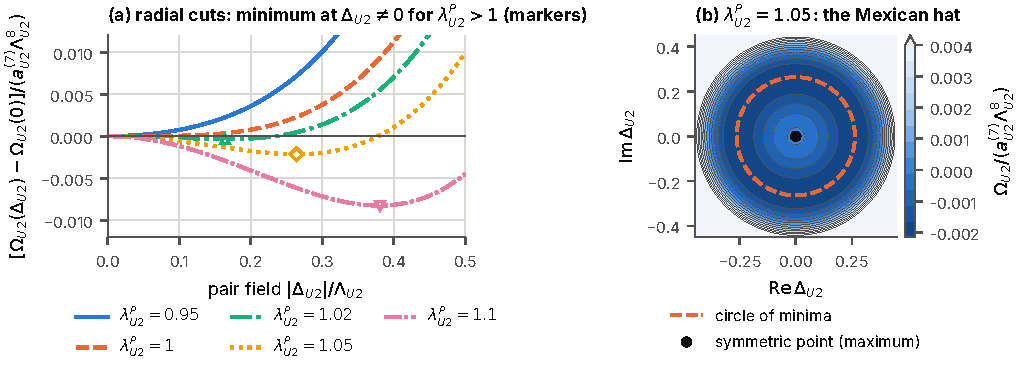
\includegraphics[width=\textwidth]{../figures/fig_r3_hat.pdf}
\caption{The effective potential in the vacuum (R7, $m_{U2}=0$, no scalar coupling), in units of
$a^{(7)}_{U2}\Lambda_{U2}^8$. (a)~Radial cuts $\Omega_{U2}(|\Delta_{U2}|)-\Omega_{U2}(0)$ for five pair
couplings; the markers are the minima. Below and at the critical coupling the minimum is at
$\Delta_{U2}=0$; above it, at $\Delta_{U2}\neq0$. (b)~The same potential at $\lambda^P_{U2}=1.05$ over
the complex plane of $\Delta_{U2}$: a maximum at the symmetric point and a circle of degenerate
minima, the Mexican hat. A point on the circle breaks $U(1)_{U2}$; all points are equivalent.}
\label{fig:hat}
\end{figure*}

\begin{figure}[t]
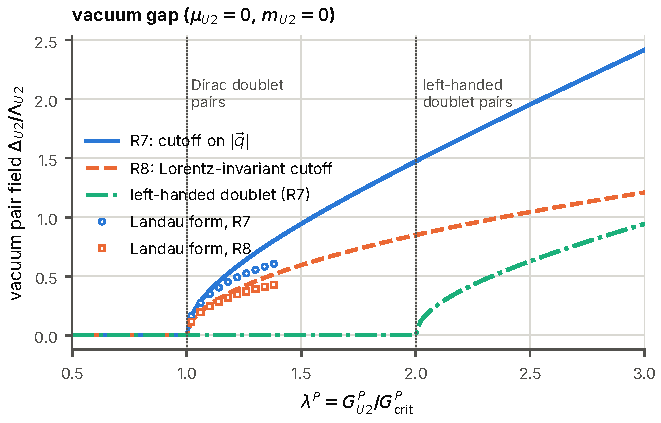
\includegraphics[width=\columnwidth]{../figures/fig_r3_gap.pdf}
\caption{The pair field at the minimum in the vacuum as a function of
$\lambda^P_{U2}=G^P_{U2}/G^{\rm crit}_{U2}$ ($m_{U2}=0$, no scalar coupling), in the two regularizations,
with the Landau forms of Eq.~\eqref{eq:landaugap} (markers) near the critical coupling.}
\label{fig:gap}
\end{figure}

\begin{table}[t]
\caption{The vacuum minimum ($m_{U2}=0$, no scalar coupling, units $\Lambda_{U2}=1$): pair field in the
two regularizations, the Landau forms of Eq.~\eqref{eq:landaugap}, and the value of the potential
at the minimum relative to $\Delta_{U2}=0$ (R7).}
\label{tab:vacuum}
\begin{ruledtabular}
\begin{tabular}{cccccc}
$\lambda^P_{U2}$ & $\Delta_{U2}$ (R7) & Landau & $\Delta_{U2}$ (R8) & Landau & $\Omega^{\min}_{U2}$ (R7)\\
\hline
{{ROWS:vacuum_gap_table}}
\end{tabular}
\end{ruledtabular}
\end{table}

\subsection{Mass against pair in the vacuum}

With $m_{U2}=0$ and both couplings, Eq.~\eqref{eq:Omega} in the vacuum reads
\begin{equation}
\Omega_{U2}=\frac{1}{G^{\rm crit}_{U2}}\Big(\frac{M^2_{U2}}{\lambda^S_{U2}}+\frac{|\Delta_{U2}|^2}{\lambda^P_{U2}}\Big)
-16\int\frac{d^7q}{(2\pi)^7}(q^2+s_{U2})^{1/2}.
\label{eq:compet}
\end{equation}
The fermion term depends on $s_{U2}=M^2_{U2}+|\Delta_{U2}|^2$ only. The reason is algebraic: the
vertices $\mathsf V^1_{U2}$ and $\mathsf V^3_{U2}$ of $\Delta_1$ (the real part of $\Delta_{U2}$) and of
$M_{U2}$ anticommute with each other and with the kinetic part (R3-A13), and so does the vertex
$\mathsf V^2_{U2}=i\,\mathrm{diag}(\mathsf 1_{16},-\mathsf 1_{16})\mathsf V^1_{U2}$ of $\Delta_2$ (the
imaginary part); at $\mu_{U2}=0$ the square of $\mathsf H_{U2}$ is then
$(q^2+M^2_{U2}+\Delta_1^2+\Delta_2^2)\mathsf 1_{32}$. At fixed $s_{U2}$ the classical part is smallest
when all of $s_{U2}$ is put into the field with the larger coupling. Hence (R3-P7, Fig.~\ref{fig:competition}):
\emph{the vacuum is a superfluid, and $U(2)_{U2}$ is broken, if and only if
$\lambda^P_{U2}>\max(1,\lambda^S_{U2})$}. For $\lambda^S_{U2}>\max(1,\lambda^P_{U2})$ the vacuum is
the massive state $(M_{U2},0)$, which breaks no gauge symmetry, and for $\lambda^P_{U2}=\lambda^S_{U2}>1$
the minima form a whole circle $M^2_{U2}+|\Delta_{U2}|^2=$ const. That degeneracy is the trace of a
larger symmetry of the massless free doublet, which rotates the mass into the pair field; the
classical part breaks it unless $G^P_{U2}=4G^S_{U2}$.

\begin{figure*}[t]
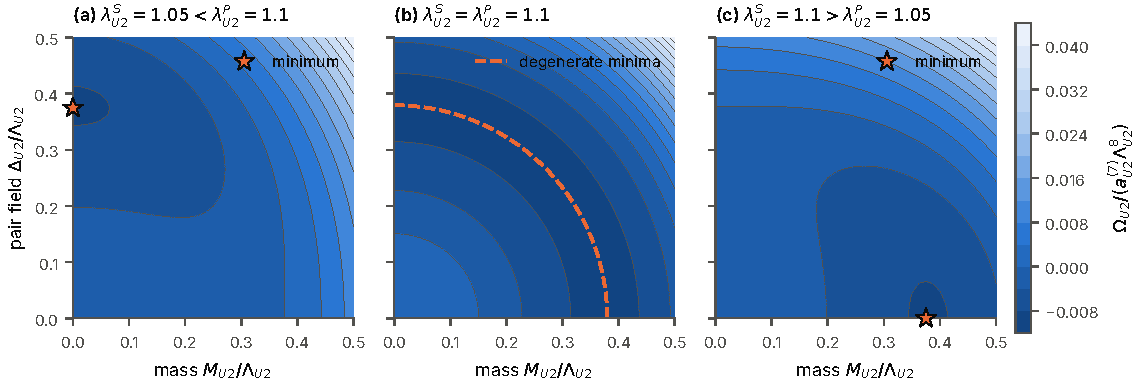
\includegraphics[width=\textwidth]{../figures/fig_r3_competition.pdf}
\caption{The vacuum effective potential (R7, $m_{U2}=0$) on the plane of the mass $M_{U2}$ and the
real pair field $\Delta_{U2}$, in units of $a^{(7)}_{U2}\Lambda_{U2}^8$, for three pairs of couplings.
(a)~$\lambda^S_{U2}<\lambda^P_{U2}$: the minimum (star) is the superfluid, $M_{U2}=0$,
$\Delta_{U2}\neq0$. (b)~$\lambda^S_{U2}=\lambda^P_{U2}$: a quarter circle of degenerate minima.
(c)~$\lambda^S_{U2}>\lambda^P_{U2}$: the minimum is the massive state, $\Delta_{U2}=0$; $U(2)_{U2}$ is
unbroken.}
\label{fig:competition}
\end{figure*}

\subsection{Finite density: every attraction pairs}

For $\mu_{U2}>M_{U2}$ the particle branch has a Fermi surface at $q=q^F_{U2}$, where
$E^-_{U2}=|\Delta_{U2}|$. Near it $dq=(\varepsilon_{U2}/q)\,d\xi^+_{U2}$, and
\begin{equation}
\begin{aligned}
4\int\frac{d^7q}{(2\pi)^7}\frac1{E^-_{U2}}&\simeq4a^{(7)}_{U2}(q^F_{U2})^6\frac{\mu_{U2}}{q^F_{U2}}\\
&\quad\times\int\frac{d\xi^+_{U2}}{[(\xi^+_{U2})^2+|\Delta_{U2}|^2]^{1/2}}\\
&\simeq8a^{(7)}_{U2}(q^F_{U2})^5\mu_{U2}\ln\frac1{|\Delta_{U2}|}
\end{aligned}
\label{eq:cooper}
\end{equation}
as $\Delta_{U2}\to0$ (R3-P8a, computed at $\Delta_{U2}=10^{-100}$ and $10^{-200}$). The right side of
the gap equation therefore grows without bound as $\Delta_{U2}\to0$, and the gap equation has a
root for \emph{every} $G^P_{U2}>0$: the Cooper instability~\cite{BCS1957}. In the
weak-coupling limit
\begin{equation}
\ln|\Delta_{U2}|=\text{const}-\frac{1}{8a^{(7)}_{U2}(q^F_{U2})^5\mu_{U2}\,G^P_{U2}},
\label{eq:bcs}
\end{equation}
the law of Bardeen, Cooper and Schrieffer in seven space dimensions: at $\mu_{U2}=0.4$ the slope of
the computed $\ln\Delta_{U2}$ against $1/G^P_{U2}$ agrees with Eq.~\eqref{eq:bcs}, ratio
${{GENM:num_BCS_ratio}}$ (R3-P9). At every $\mu_{U2}>0$ of a scan of 60 values and at every coupling
tested, $\lambda^P_{U2}\in\{0.5,0.8,0.95,1.05\}$, the minimum has $\Delta_{U2}>0$ (R3-P8); where the
gap is below $10^{-300}$, the smallest positive number of the arithmetic, its logarithm follows from
Eq.~\eqref{eq:cooper}. Figure~\ref{fig:density} shows both results, and Fig.~\ref{fig:phase} the gap
on the plane of the coupling and the chemical potential. The number density
$n_{U2}=-\partial\Omega_{U2}/\partial\mu_{U2}=8\int d^7q/(2\pi)^7[(\varepsilon_{U2}+\mu_{U2})/E^+_{U2}
-(\varepsilon_{U2}-\mu_{U2})/E^-_{U2}]$ of the superfluid agrees with the derivative of
$\Omega^{\min}_{U2}$ computed by differences (R3-P11); no derivative of $\Delta_{U2}$ is needed,
because $\Omega_{U2}$ is stationary in $\Delta_{U2}$.

\begin{figure*}[t]
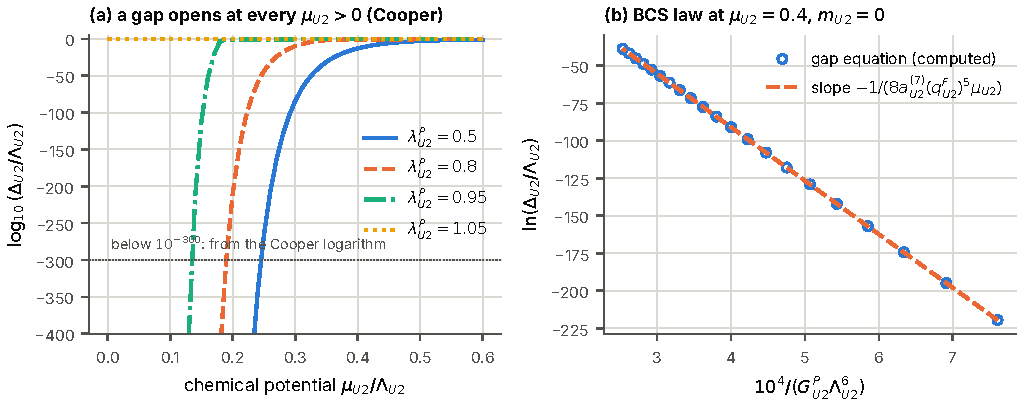
\includegraphics[width=\textwidth]{../figures/fig_r3_density.pdf}
\caption{Pairing at finite density (R7, $m_{U2}=0$, no scalar coupling). (a)~$\log_{10}\Delta_{U2}$
at the minimum against $\mu_{U2}$ for four pair couplings, three of them below the critical coupling
of the vacuum: a gap opens at every $\mu_{U2}>0$; below $10^{-300}$ the logarithm is computed from
Eq.~\eqref{eq:cooper}. (b)~The law of Eq.~\eqref{eq:bcs} at $\mu_{U2}=0.4$: $\ln\Delta_{U2}$ against
$1/G^P_{U2}$ (circles) and the predicted slope (dashed).}
\label{fig:density}
\end{figure*}

\begin{figure}[t]
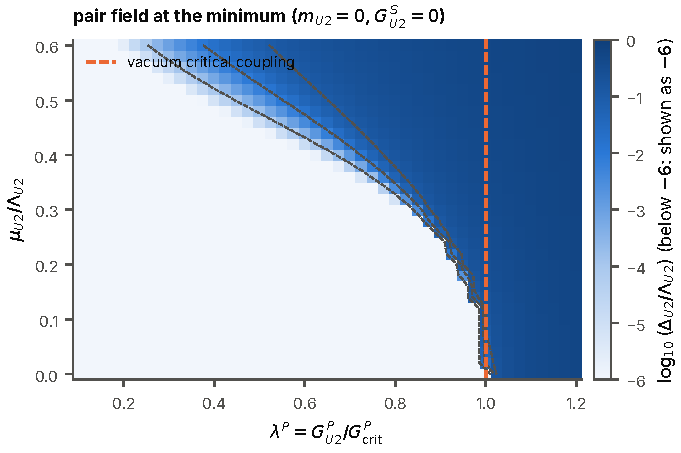
\includegraphics[width=\columnwidth]{../figures/fig_r3_phase.pdf}
\caption{$\log_{10}\Delta_{U2}$ at the minimum on the plane of $\lambda^P_{U2}$ and $\mu_{U2}$ (R7,
$m_{U2}=0$, no scalar coupling), with contour lines at $-4$, $-2$, $-1$. Values below $10^{-6}$ are
shown as $10^{-6}$: the light region has a gap too, exponentially small by Eq.~\eqref{eq:bcs}. The
dashed vertical line is the critical coupling of the vacuum.}
\label{fig:phase}
\end{figure}

\subsection{Breaking of the gauge group driven by density}

If the scalar coupling is the stronger one, $\lambda^S_{U2}>\lambda^P_{U2}>1$, the vacuum is the
massive state, and $U(2)_{U2}$ is unbroken. For $\lambda^S_{U2}=1.1$ and $\lambda^P_{U2}=1.05$ its mass
is $M_{U2}={{GENM:num_transition_M0}}$. While $\mu_{U2}<M_{U2}$ there are no states to fill, and the
potential of the massive state does not change with $\mu_{U2}$; the superfluid, in contrast, lowers
its potential as $\mu_{U2}$ grows. At $\mu_{U2}\approx{{GENM:num_mu_transition}}$ the global minimum
jumps from the massive symmetric state to the superfluid with $M_{U2}=0$ (R3-P10,
Fig.~\ref{fig:transition}); at $\mu_{U2}=0.6$ the pair field is ${{GENM:num_transition_Dend}}$. The
transition is of first order: $M_{U2}$ and $\Delta_{U2}$ jump. The breaking
$U(2)_{U2}\to SU(2)_{U2}$ is then driven by the density, not by the strength of the coupling.

\begin{figure*}[t]
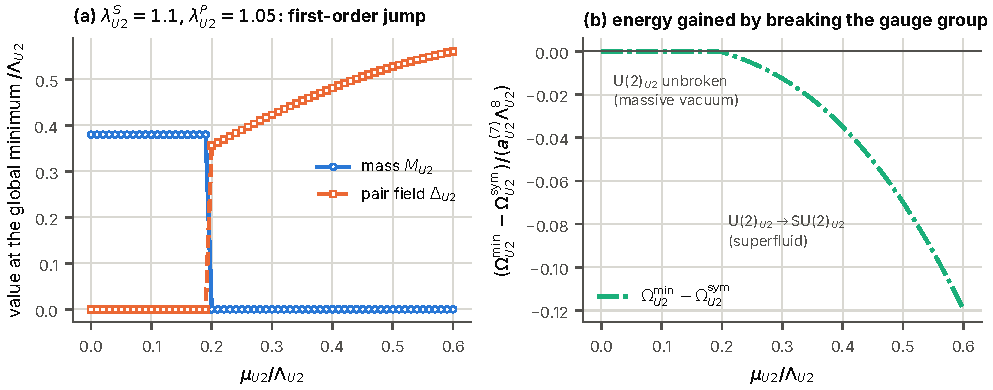
\includegraphics[width=\textwidth]{../figures/fig_r3_transition.pdf}
\caption{Breaking of $U(2)_{U2}$ driven by density, $\lambda^S_{U2}=1.1$, $\lambda^P_{U2}=1.05$, $m_{U2}=0$
(R7). (a)~Mass and pair field at the global minimum against $\mu_{U2}$: a jump at
$\mu_{U2}\approx{{GENM:num_mu_transition}}$. (b)~The potential at the global minimum relative to the
lowest state with $\Delta_{U2}=0$, in units of $a^{(7)}_{U2}\Lambda_{U2}^8$: zero while the symmetric
state is the ground state, negative after the transition.}
\label{fig:transition}
\end{figure*}

\subsection{The chiral doublet}
\label{sec:chiral}

A doublet of left-handed fields has no mass term (Sec.~\ref{sec:pairs}) and cannot carry the gauged
$U(1)_{U2}$ (Sec.~\ref{sec:gauge}), but it can pair. Its Nambu spinor has 16 components, the
left-handed $\psi^1_{U2}$ and the conjugate of the left-handed $\psi^2_{U2}$, which is right-handed;
with $C^+_{1671}$ the eigenvalues are $\pm[(q\mp\mu_{U2})^2+|\Delta_{U2}|^2]^{1/2}$, each fourfold
(R3-C5): half the states of the Dirac doublet. Its potential at the coupling $G^P_{U2}$ is half
that of the Dirac doublet at $G^P_{U2}/2$, so in the vacuum it pairs only for
$G^P_{U2}>2G^{\rm crit}_{U2}$ ($180\pi^4\Lambda_{U2}^{-6}$ in R7), while at finite density it pairs for
any attraction (R3-P12, with a nonzero gap at $\lambda^P_{U2}=0.8$, $\mu_{U2}=0.4$).
